\documentclass[letterpaper,12pt]{article}


\listfiles


%\usepackage{setspace}
%\doublespacing
\usepackage{pdfcomment}
%usepackage{hyperref}
\hypersetup{hidelinks}

%%  Accepte les caractères accentués dans le document (UTF-8).
\usepackage[utf8]{inputenc}
%\usepackage[french]{babel}
\usepackage[T1]{fontenc}

\usepackage[bb=boondox]{mathalfa}






%change les references aux equations
%\let\oldref\ref
%\renewcommand{\ref}[1]{\in@{eq:}{#1} \ifin@ (\oldref{#1}) \else \oldref{#1} \fi}

%commentaires
\usepackage{verbatim}

%double espacement
\usepackage{setspace}
% \doublespacing

%notes sur le pdf


%------------------------------
%packages pour tableaux
\usepackage[table,xcdraw]{xcolor}
\usepackage{rotating}


%-----------------------------

%packages pour figures
%\usepackage{fancybox}
\usepackage{epsfig}
\usepackage{graphicx}


%------------------------------------------------
%Bibliographie

%ancienne
%\usepackage[round]{natbib}
%\usepackage{numcompress}
%\bibliographystyle{model4-names}

% Natbib setup for author-year style
\usepackage{natbib}
\bibpunct[, ]{(}{)}{,}{a}{}{,}%
\def\bibfont{\small}%
\def\bibsep{\smallskipamount}%
\def\bibhang{24pt}%
\def\newblock{\ }%
\def\BIBand{and}%
\bibliographystyle{informs2014trsc}


%\usepackage[strings]{underscore}
%\bibliographystyle{plainnat}
%------------------------------------------------

%-----------------------------------------
%TIKZ
\usepackage{tikz}
\usetikzlibrary{arrows,shapes,positioning,shadows,trees}
\usetikzlibrary{patterns}
\usetikzlibrary{calc, graphs}


\tikzset{hide on/.code={\only<#1>{\color{fg!20}}}}
\tikzset{
	invisible/.style={opacity=0},
	visible on/.style={alt=#1{}{invisible}},
	alt/.code args={<#1>#2#3}{%
		\alt<#1>{\pgfkeysalso{#2}}{\pgfkeysalso{#3}} % \pgfkeysalso doesn't change the path
	},
} 
\tikzset{
	depnode/.style={circle, minimum size=0.3cm, draw, thin},
	arrnode/.style={circle, minimum size=0.3cm, draw, thin, fill=black},
	waitnode/.style={circle, minimum size=0.3cm, draw, thin, pattern = north east lines},
	sourcesinknode/.style={circle, draw, minimum size=0.3cm, line width=0.1cm},
	wait/.style={->, >=triangle 45, thin},
	nullarc/.style={->, >=open triangle 45, thin},
	flight/.style={->, >=stealth, thin},
	deadhead/.style={->, >=stealth, thin, bend left=10, dashed},
	connect/.style={->, >=open diamond, thin},
	rest/.style={->, >=diamond, thin},
	begend/.style={->, >=stealth, thick, dotted}
}
%-------------------------------------------


%packages de math
\usepackage{amssymb}
\usepackage{amsmath}

\usepackage{caption}

%packages divers
\usepackage{enumerate}
\usepackage[top=1in, bottom=1in, left=1in, right=1in]{geometry}

%packagespour tableaux
\usepackage{multirow}
%\renewcommand{\arraystretch}{0.6}

%packages et commande pour décrire les algorithmes
%\usepackage{algorithm}
%\usepackage{algorithmicx}
%\usepackage{algpseudocode}

%packages pour bibliographie

%% Vancouver numbered
%\usepackage{numcompress}\bibliographystyle{model3-num-names}
%\usepackage{natbib}
%\usepackage{bibentry}

%couleur
\usepackage{color}



%commandes personnalisées

%mettre parentheses automatiquement aux references
\let\oldref\ref
\makeatletter
\newcommand\myref[1]{\oldref{#1}}
\makeatother
%les accolades supplémentaires sont pour que tout soit inclus dans les commandes comme les exposants (on peut faire $x^\ref{...}$)
\renewcommand{\ref}[1]{{\myref{#1}}}
\renewcommand{\eqref}[1]{{(\myref{#1})}}

\renewcommand*{\thesubsection}{Question \arabic{section}.\arabic{subsection}}



\newcommand{\red}[1]{{\color{red}[#1]}}
\newcommand{\new}[1]{{\bfseries#1}}
\usepackage[breakable]{tcolorbox}
\newcommand{\nouveau}[2][]{
	\begin{center}
		\begin{tcolorbox}[left=0pt, right=0pt, boxsep=5pt, width=1.03\textwidth, colframe=red!75!black,title={\textbf{\Large Nouveau! #1}},coltitle=black, colbacktitle=white, colback=white, breakable]
			#2
			
		\end{tcolorbox} 
	\end{center}
}

\newcommand{\note}[1]{\red{#1}}

%\renewcommand{\baselinestretch}{1.5} 

\title{ Optimisation de la production d'une mine à ciel ouvert }
\author{\textsc{\large{Frédéric Quesnel}} \\ MTH6601}

%\date{\today}

%\baselineskip=15pt

\begin{document}
	
	\maketitle
	
	\tableofcontents
	
	\setcounter{section}{-1}
	
	%========================================================================================
	% Section 0
	%========================================================================================
	\section{Avant de commencer...}
	Ce TP concerne l'optimisation des opérations d'une mine à ciel ouvert. Il est basé sur un vrai projet de recherche mené par un professeur de Polytechnique. Dans ce TP, vous étudirez un modèle simplifié de mine à ciel ouvert à l'aide d'un simulateur. Une présentation décrivant le fonctionnement de la mine et du simulateur se trouve sur Moodle. Il est fortement recommandé de relire ce document avant de commencer. Pour toute question concernant le simulateur ou cet énoncé, ou encore pour signaler un bogue du simulateur, n'hésitez pas à contacter à Frédéric Quesnel. 
	
	
	Il est encouragé d'inclure des tableaux ou des graphiques pertinents à vos réponses. Toutefois, le coeur de l'évaluation portera sur la justesse de votre analyse et vos conclusions. 
	
	
	%========================================================================================
	% Section 1 Prediction des temps de parcours
	%========================================================================================
		
		\section{Prédiction des temps de parcours}

	Le temps de parcours d’un camion sur un chemin varie de manière stochastique, et peut être influencé par divers facteurs tels que l’état de la route ou la météo. Il est important d'être en mesure d'estimer correctement ces temps de parcours afin de bien planifier les opérations. Dans cette section, vous étudierez trois formules qui peuvent être utilisées pour estimer les temps de parcours. 
	
	Lorsqu'un camion débute un trajet, la formule de prédiction estime son temps de parcours. Il s'agit du \textit{temps de parcours prédit}. Lorsque le camion arrive à sa destination, son \textit{temps de parcours observé} est enregistré. Dams le simulateur, le graphe \textit{Temps de parcours observés et prédits} affiche les temps observés et prédits des camions sur plusieurs chemins spécifiques (la légende indique de quels chemins il s'agit).
	
	
	Soient $t_{ij}^k$ et $t^{*k}_{ij}$ les temps prédits et observés pour le segment (chemin) $(i,j)$ à l'instant $k$. $t_{ij}^{k-1}$ et $t^{*k-1}_{ij}$ dénotent les temps prédits et observés du dernier camion sur le segment $(i, j)$ à être arrivé avant l'instant $k$. Soit $A$ l'ensemble des segments. Le logiciel de simulation propose les trois formules suivantes pour estimer le temps de parcours d’un camion sur le segment $(i,j)$ : 
	
	
	\begin{itemize}
		
		\item Moyenne des observations précédentes (sur le même segment)
		
		\begin{equation}
		t_{ij}^k = \frac{1}{n} \sum\limits_{k=1}^n t_{ij}^{*k-1}
		\end{equation}
		
		\item Combinaison convexe
		
		\begin{equation}
		t_{ij}^k = \lambda t^{*k-1}_{ij} + (1-\lambda) t_{ij}^{k-1} \qquad \lambda \in [0, 1]
		\end{equation}
		
		\item Erreur précédente
		
		\begin{equation}
		t_{ij}^k = \lambda t^{*k-1}_{ij} + (1-\lambda) t_{ij}^{k-1} \left( 1- \frac{\sum\limits_{(l,m) \in A} t_{lm}^{k-1} - t_{lm}^{*k-1}}{\sum\limits_{(l,m) \in A} t_{lm}^{*k-1}}\right)
		\end{equation}
		
		
	\end{itemize}
	
	L'interface permet de modifier les valeurs de $n$ et $\lambda$ pour chaque formule.
	
	\vspace{10pt}
	\noindent \textbf{\Large Protocole expérimental: }
	
	\begin{itemize}
		\item Mine : 4 pelles
		\item Nombre de camions de 60 tonnes : 20
		\item Nombre de camions de 100 tonnes : 0
		\item Temps de simulation : 24h
		\item Fonction de score : « aléatoire » (option par défaut)
	\end{itemize}
	
	\vspace{10pt}
	\noindent \textbf{\large Étapes de simulation :  }
	
	\begin{enumerate}
		\item Lancer la simulation à l’aide du bouton play (pour voir l’animation).
		\item Attendre au moins 3h de simulation (pour que les formules de prédictions se stabilisent).
		\item Varier la température (de neige à soleil, ou l’inverse).
		\item Attendre que la formule de prédiction se stabilise de nouveau, ou la fin de la simulation.
	\end{enumerate}
	
	
	
	\subsection{Caractéristiques d'une "Bonne" fonction de prédiction }

 	Les trois fonctions ci-dessus adaptent leurs prédictions en se basant sur les observations précédentes. Donnez deux comportements désirables d'une formule de prédiction.

	\begin{comment}
	\textbf{Réponse : }
	
	\begin{itemize}
		\item Bonne valeur de prédiction en régime stable.
		\item S'adapte rapidement aux changements de conditions.
		\item Peu sensible aux données aberrantes (ex. si un camion tombe en panne).
	\end{itemize} 
	\end{comment}
	%L’objectif est de trouver une formule de prédiction qui réagit rapidement lors de changements drastiques des conditions de conduites sur l’ensemble de la mine.
	
	
	
	
	
	
	\subsection{Étude des formules}
	\label{sec:pred:etude}
	\begin{enumerate}[a)]
		\item Observez le comportement de la formule « Moyenne des observations précédentes » avec différentes valeurs de $n$. Quels sont les avantages et les inconvénients à utiliser une plus grande valeur de $n$. 
		\item En utilisant la formule « combinaison convexe », on observe que plus la valeur de $\lambda$ est grande, plus la formule s’adapte rapidement aux changements de température. Doit-on conclure qu’il vaut mieux utiliser $\lambda=1$? Pourquoi?
		\item La formule « Erreur précédente » est celle qui s’adapte le plus rapidement aux changements de conditions météorologiques. Comment expliquez-vous ce phénomène? 
		\item Si d’autres facteurs que la météo affectaient le temps de déplacement (par exemple, la détérioration soudaine d'une route), la formule "erreur précédente" serait-elle encore valide? Justifiez.
		\item En général, les formules de prédiction semblent plus précises sur le chemin \textit{concentrateur:pelle1} que sur le chemin \textit{sterile:pelle3}. Comment expliquez-vous cela?	
	\end{enumerate}

	\red{Dans la version précédente, la question \ref{sec:pred:etude} était séparée en quatre questions.}	
	
	\subsection{Temps avant le début du remplissage}
	
	Pour cette question, supposez que les temps de transport et de remplissage sont déterministes. Supposons que $n$ camions sont en route pour la pelle et que $m$ camions sont déjà en attente à celle-ci. Soit $t_i$ le temps que prend le camion $i$ pour arriver à la pelle, en secondes, et supposons que les camions sont ordonnés par ordre de temps d'arrivée à la pelle ($t_1 \leq t_2 \leq ...\leq t_{n-1} \leq t_n$). Un camion est en cours de remplissage, et ce remplissage sera complété dans $t^r$ secondes. Le temps de remplissage d'un camion est de $T^R$ secondes. Cette situation est illustrée sur la figure \ref{fig:file}.
	
	\begin{figure}
		\center
		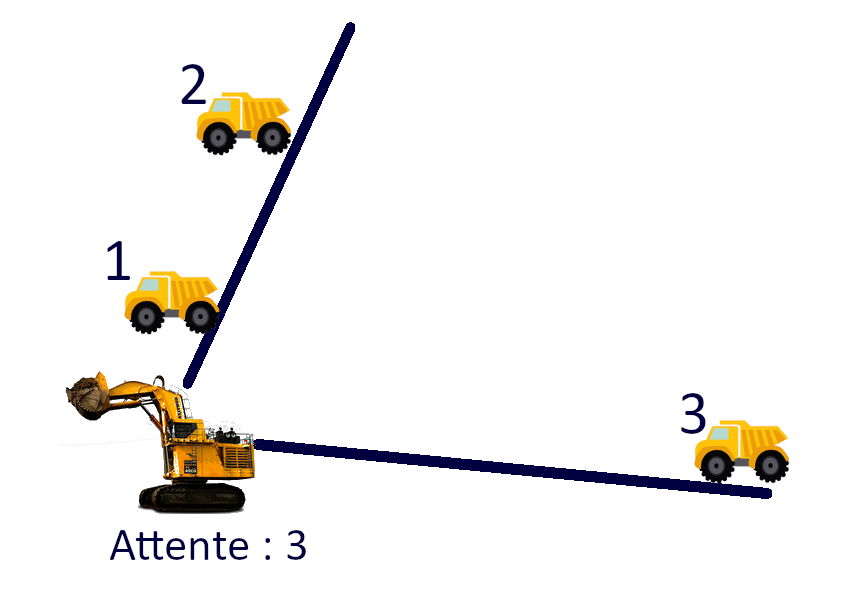
\includegraphics[width=0.4\linewidth]{File.png}
		\caption{\label{fig:file}}
	\end{figure}
	
	Donnez une formule permettant de calculer dans combien de temps débutera le remplissage du camion $n$.
	
	\textbf{Indice :} Il peut s'agir ou non d'une fonction définie par récurrence.
	

	%===========================================================================
	% Section 2 Affectation des camions pour maximiser la production
	%===========================================================================
	
	 \section{Affectation des camions pour maximiser la production}
\label{sec:score}

Dans cette section, nous souhaitons maximiser la production totale (minerai + stérile) de la mine. Pour ce faire, il vous faudra développer les stratégies pour prendre les décisions suivantes : 

\begin{enumerate}
	\item \textbf{Affectation à une pelle : }Lorsqu'un camion vient de se faire décharger (à un concentrateur ou une pelle) et devient disponible, à quelle pelle doit-il aller se faire remplir?
	\item \textbf{Choix de la station de décharge : }Lorsqu'une pelle termine de charger un camion, vers quelle station (stérile ou concentrateur) doit aller se faire décharger le camion? 
\end{enumerate}



\vspace{10pt}
\noindent \textbf{\Large Protocole expérimental: }

\begin{itemize}
	\item Mine : 10 pelles
	\item Nombre de camions de 60 tonnes : 20
	\item Nombre de camions de 100 tonnes : 20
	\item Temps de simulation : 24h
\end{itemize}


\vspace{10pt}
\noindent \textbf{\large Étapes de simulation :  }
\begin{enumerate}
	\item Lancer la simulation (à l'aide du bouton \textit{play}, ou \textit{compléter auto)}.
	\item Enregistrer les résultats.
\end{enumerate}

\noindent\textbf{Astuces : }

\begin{itemize}
	\item N'hésitez pas à utiliser la mine à 4 pelles, ou un nombre moins élevé de camions pour déboguer vos fonctions de score!
	\item Rappelez-vous que certains éléments de la simulation sont aléatoires! Exécutez chaque simulation plusieurs fois afin d'obtenir des résultats statistiquement significatifs.
\end{itemize}



%-------------------------------------
% fonction de score
%-------------------------------------
\subsection{Affectation à une pelle à l'aide d'un algorithme glouton} 
\label{max_prod:score}

Une première façon de contrôler l'affectation des camions est via un algorithme glouton qui affecte les camions un à un. Lorsqu'un camion devient disponible, on calcule un \textit{score} pour chaque pelle, correspondant à l'utilité d'affecter le camion disponible à la pelle. Le logiciel assigne ensuite le camion à la pelle ayant le plus petit score. En cas d'égalité, la pelle avec le plus petit numéro est choisie. Vous pouvez définir la fonction de score utilisée en modifiant le champ \textit{fonction de score} de l'interface graphique. 

Élaborez une fonction de score qui maximise la production de la mine. Votre fonction de score peut contenir toutes les variables fournies dans la section \ref{sec:vars}, ainsi que les opérations élémentaires (+, -, *, /, \%). Les exposants peuvent également être utilisés à l'aide de la fonction Java (\verb!Math.pow([base], [exopsant]!). Par exemple, entrer la formule "n1" envoie toujours un camion disponible à la pelle ayant le moins de camions en attente.

\vspace{10pt} 
\noindent\textbf{Dans votre réponse,}  
\begin{itemize}
	\item Indiquez la fonction de score choisie.
	\item Expliquez le raisonnement derrière votre fonction de score.
	\item Comparez la production obtenue avec votre formule d'assignation avec celle d'une assignation aléatoire (écrivez "aléatoire" dans le champ \textit{fonction de score}).
\end{itemize}


%--------------------------------------
% Avec code
%--------------------------------------
\begin{comment}
\subsection{Décisions d'affectation à l'aide de règles complexes} 
\label{max_prod:code}


Vous devez maintenant programmer des règles de décision plus complexes en modifiant la classe CustomDecisionMaker. Plus précisément, 

\begin{itemize}
	\item Modifiez les fonctions \verb!computeDecisionScore! et \verb!computeCustomDecisionScore! pour créer une fonction de score pour l'affectation de camions aux pelles.
	\item Modifiez les fonctions \verb!selectReturnStation! et \verb!customSelectReturnStation! pour choisir vers quelle station de déchargement (quel stérile ou concentrateur) un camion ira se faire décharger.
\end{itemize}

\red{Peut-être seulement le deuxième point. Le premier point est redondant avec une question de la section suivante...}

\vspace{10pt}
\noindent\textbf{Dans votre réponse,} 

\begin{itemize}
	\item Décrivez brièvement vos algorithmes.
	\item Comparez la production obtenue avec votre formule d'assignation vos résultats de la question \ref{max_prod:score}.
\end{itemize}
\end{comment}

%---------------------------------------------
% deux types de camions
%---------------------------------------------
\subsection{Deux types de camions}
Certains camions étaient vieux et ont été remplacés par des camions nouvelle génération. Ceux-ci sont plus lents, mais ont une capacité de 100 tonnes.

Proposez une fonction de score différente pour chaque type de camion. Répondez aux mêmes questions qu'à la question \ref{max_prod:score}.

\textbf{Indice : }Pour vous aider à élaborer vos fonctions de score, posez-vous les questions suivantes : 
\begin{itemize}
	\item Dans quelle situation as-t-on avantage à utiliser un camion plus rapide?
	\item Quel type de camion as-t-on avantage à envoyer aux pelles éloignées et peu visitées?
\end{itemize}

%---------------------------------------------
% Affectation
%---------------------------------------------
\subsection{Problème d'affectation}

Vous pouvez également prendre les décisions d'affectation en résolvant le problème d'affectation suivant : 

\red{TODO écrire le problème}

On assigne le camion qui nous intéresse selon la solution du problème, et on écarte le reste de la solution. Pour activer cette fonctionnalité, entrez \red{optimise\_production} dans le champ \textit{fonction de score}.

\vspace{10pt}
\noindent\textbf{Dans votre réponse,} 

\begin{itemize}
	\item Donnez un exemple hypothétique pour lequel il est avantageux d'utiliser un problème d'affectation par rapport à assigner les camions un par un.
	\item Comparez la production obtenue avec le problème d'affectation avec ceux de la question \ref{max_prod:score}. 
	\item Comment expliquez-vous les résultats obtenus?
\end{itemize}
\red{Selon mes tests, ici le problème d'affectation marche moins bien que la façon "1 camion à la fois". C'est parce que la fonction objectif minimise le temps d'attente des pelles, ce qui n'est pas toujours optimal. Par exemple, il peut être préférable d'envoyer les camions à une pelle plus proche quitte à laisser attendre une pelle éloignée. Il n'est pas évident de trouver une fonction objectif qui fait ce que l'on veut sans effets pervers. En gros, il faut s'assurer que ce qui est avantageux pour le camion qui nous intéresse ne soit pas plus avantageux pour un camion qui deviendra disponible plus tard. }






	%===========================================================================
	% Section 3 Affectation des camions pour atteindre des objectifs de production
	%===========================================================================
	
	 %---------------------------------------------------------------------------------------------------------
\section{Affectation des camions pour atteindre des objectifs de production}
\label{sec:objectifs}

Dans la réalité, maximiser la production totale n'est pas toujours souhaitable. En effet, extraire du stérile ne rapporte pas d'argent à court terme. De plus, il faut que le minerai amené au concentrateur soit d'assez bonne qualité : il doit contenir une quantité suffisante de fer, mais pas trop d'impuretés (ici le soufre). Dans cette section, nous allons développer des stratégies pour maximiser la production sous ces contraintes.


\vspace{10pt}
\noindent \textbf{\Large \textbf{Objectif et contraintes de production} } 

\noindent Soit :

\begin{itemize}
	\item $x_c$ : Quantité livrée aux concentrateurs.
	\item $x_s$ : Quantité livrée aux stériles.
	\item $y_{fe}$ : Taux de fer (\%) dans le minerai aux concentrateurs.
	\item $y_{s}$ : Taux de soufre (\%) dans le minerai aux concentrateurs.
\end{itemize}


\begin{itemize}
	\item \textbf{Objectif : } Maximiser $x_c + 0.2 x_s$.
	\item \textbf{Contrainte sur la quantité de stérile : } 
	
	\[x_s \leq 0.25 (x_c+x_s)\]
	
	\item \textbf{Taux de fer : } Entre 26\% et 27\%.
	\[ 26 \leq y_{fe} \leq 27\% \]
	
	\item \textbf{Taux de soufre : } 
	
	\[y_s \leq 1.9\]
\end{itemize}

\vspace{10pt}
\noindent \textbf{\Large \textbf{Protocole expérimental }} 
\begin{itemize}
	\item Mine : 10 pelles
	\item Nombre de camions de 60 tonnes : 20
	\item Nombre de camions de 100 tonnes : 0
	\item Temps de simulation : 24h
\end{itemize}


%----------------------------------------
%avec code 
\subsection{Stratégies d'affectation dynamique}
\label{max_cont:code}

Vous devez maintenant programmer des règles de décision plus complexes en modifiant la classe CustomDecisionMaker. Plus précisément, 

\begin{itemize}
	\item Modifiez les fonctions \verb!computeDecisionScore! et \verb!computeCustomDecisionScore! pour créer une fonction de score pour l'affectation de camions aux pelles.
	\item Modifiez les fonctions \verb!selectReturnStation! et \verb!customSelectReturnStation! pour choisir vers quelle station de déchargement (quel stérile ou concentrateur) un camion ira se faire décharger.
\end{itemize}

Votre algorithme doit être dynamique, c'est à dire que les décisions prises doivent dépendre de l'état de la mine. Vous devez tenter de maximiser les objectifs de production tout en respectant les contraintes.

\vspace{10pt}
\noindent\textbf{Dans votre réponse,} 

\begin{itemize}
	\item Décrivez brièvement vos algorithmes. Expliquez le raisonnement derrière ceux-ci.
	\item Donnez les résultats d'une simulation (quantités produites, respect des contraintes, etc.).
\end{itemize}



%----------------------------------------
%avec plan + problème d'affectation
\subsection{Plan + problème d'affectation}

Tel que présenté dans les diapositives sur Moodle, on peut également définir un \textit{plan d'opération} qui permettra de respecter les contraintes. On peut ensuite affecter les camions en tenant compte des prochains camions qui seront disponibles en résolvant un problème d'affectation qui tente de respecter le plan le plus possible. Vous pouvez activer cette option en entrant la commande \red{"optimise\_plan"} dans le champ \textit{fonction de score}.

\vspace{10pt}
\noindent\textbf{Dans votre réponse,}  

\begin{itemize}
	\item Comparez la production obtenue à l'aide du problème d'affectation avec vos résultats de la question \ref{max_cont:code}.
	\item Dans quelle mesure le problème d'affectation arrive-t-il à suivre le plan? Qu'est-ce qui peut expliquer les écarts observés? \red{Un peu vague comme question?}
\end{itemize}



%--------------------------------------------
\subsection{} 


Assignez les camions un par un en utilisant la même fonction objectif que dans le problème d'affectation ($c_{ij} = \left(E(AC)-AC\right)^2 + \left(E(AP)-AP\right)^2$, voir présentation sur Moodle). Pour ce faire, entrez la commande \red{"optimal\_assign"} dans le champ \textit{fonction de score}. 

\noindent Vous devriez constater que cette stratégie fonctionne très mal. Expliquez pourquoi.

\noindent\textbf{Indice : }Dans votre explication, il est suggéré d'utiliser un petit exemple théorique avec deux pelles et deux camions.



	
	%===========================================================================
	% Section 4 Modification du plan d'opération
	%===========================================================================
	
	\section{Modification du plan d'opération}

Le plan d'opérations peut être modifié dans le but d'atteindre divers objectifs de production. Pour modifier la cible d'une pelle, effectuez un clic droit sur la pelle, cliquez sur "Modifier le plan", et entrez la valeur désirée. Pour remettre les valeurs par défaut, chargez la mine de nouveau.

Protocole expérimental 

•Mine : 10 pelles

•Nombre de camions de 60 tonnes: 20

•Nombre de camions de 100 tonnes: 20

•Temps de simulation : 24h

•Fonction de score : optimise ou optimalassign.

\subsection{Estimation de production}

Supposez que le plan par défaut est suivi à la lettre. Estimez quelle devrait être, sur une période de 24h : 

•La quantité de minerai livrée au concentrateur.

•La quantité de stérile livrée à la pile de stérile.

•Le pourcentage de fer et de soufre au concentrateur.

Comparez ces chiffres avec les résultats d'une simulation. Comment expliquez-vous la différence observée?

\subsection{Modification manuelle du plan}

Un nouveau client souhaite acheter du minerai de très bonne qualité (et à payer cher pour!). Il lui faut au moins X tonnes de minerais d'ici 24 heures! Les nouveaux objectifs et contraintes de production sont : 

•Objectif : Maximiser (on priorise davantage la production de minerai).

•Quantité de minerai : 

•Taux de fer : 

•Taux de soufre : 

Proposez un plan d'opération qui permet de respecter toutes les contraintes (dans une simulation). Simulez ce plan et donnez-en les caractéristiques de production.

\subsection{Optimisation du plan}

En supposant que n'importe quel plan peut être suivi à la lettre, écrivez un modèle d'optimisation linéaire qui détermine le meilleur plan d'opérations en régime continu. Utilisez les mêmes objectifs et contraintes que pour la section 

À l'aide d'un logiciel d'optimisation (le solveur d'Excel, par exemple), résolvez ce problème et donnez sa solution. Selon votre plan, estimez :

•La quantité de minerai livrée au concentrateur.

•La quantité de stérile livrée à la pile de stérile.

•Le pourcentage de fer et de soufre au concentrateur.

Plan "optimal" en pratique

Simulez le plan trouvé en 4.2. 

Dans votre réponse, 

•Comparez les résultats de la simulation avec vos prédictions de la question . Expliquez les différences observées ( autrement dit, quels sont les éléments que le modèle d'optimisation linéaire ne considère pas?).

•Les modèles linéaires ont tendance à produire des solutions extrêmes. Expliquez en quoi cela pourrait être un problème avec le modèle développé en .

\subsection{Ajustement dynamique du plan}

Il arrive qu'une pelle subisse un bris mécanique et tombe en panne pour une durée indéterminée. Il faut alors ajuster le plan afin de maintenir le respect des objectifs de production. Lorsqu'une pelle redevient fonctionnelle, il faut à nouveau réajuster le plan. Il se peut également que plusieurs pelles soient en panne simultanément.

Vous devez développer une stratégie de mise à jour du plan. Pour ce faire, modifiez les fonctions et de la classe .

Testez votre stratégie en simulant 10 jours sur la mine 10 pelles. Utilisez le problème d'affectation pour assigner les camions (option optimiseplan).

Il faut simuler 10 jours pour qu'il y ait assez de pannes pour que les résultats soient statistiquement significatifs.

Dans votre réponse, 

•Décrivez brièvement votre stratégie de mise à jour du plan.

•Donnez les résultats pertinents de la simulation.

•Comparez vos résultats avec une simulation de 10 jours avec un plan fixe. 

Bonus (?) : Si la stratégie utilise un modèle de programmation linéaire.

	
	%===========================================================================
	% Section 5 Optimisation des coûts de production + bonus
	%===========================================================================
		\section{Optimisation des coûts de production}
	%---------------------------------------------------------------------------------------------------------
	
	Si le coût pour une minute d’attente d’une pelle est 10\$, que l’attente d’un camion de 60 tonnes coûte 3\$/minute, et que l’attente d’un camion de 60 tonnes coûte 5\$/minute, estimez empiriquement le nombre optimal de camions de chaque type? Utilisez le plan par défaut.
	
	

	\section{Liste des variables}
	\label{sec:vars}
	
	
	\begin{itemize}
		\setlength\itemsep{0.01em}
		\item $x1$ : Vitesse moyenne d'un camion.
		\item $x2$ : Vaut 1 si la pelle est actives, 0 sinon.
		\item $x3$ : Nombre réel aléatoire entre 0 et 1.
		\item $x4$ : Infini ($(2-2^{-52})*2^{1023}$)
		\item $t1$ : Temps moyen de remplissage d'un camion.
		\item $t2$ : Temps de parcours espéré jusqu'à la pelle.  
		\item $d1$ : Distance entre le camion et la pelle.
		\item $n1$ : Nombre de camions en attente (sans compter le camion en remplissage).
		\item $n2$ : Nombre de camions à la pelle (en comptant le camion en remplissage).
		\item $n3$ : Nombre de camions en route pour la pelle.
		\item $t3$ : Temps espéré avant que la pelle n'ait terminé le remplissage des camions actuellement en attente.
		\item $t4$ : Temps espéré avant le début du remplissage du camion.
		\item $t5$ : Temps d'attente espéré du camion (0 si la pelle est inactive quand le camion arrive).
		\item $t6$ : Temps d'attente espéré de la pelle (peut être négatif si le camion arrive avant que la pelle ne soit en attente).
	\end{itemize}
	
	
	
\end{document}

